\section{Ergebnisse}

Die Verwendung neuer Wegtypen konnte erfolgreich eingebunden werden wie in Abbildung \ref{fig:footway} zu erkennen ist.
Hier wurden als Zielpunkte verschieden Stellen auf der Fußgängerzone(v.a. Hauptstraße) in der Heidelberger Altstadt\footnote{Heidelberg liegt natürlich nicht in Schwaben.
Für diesen Test wurde ein Gebiet um Heidelberg als Datengrundlage verwendet.} gewählt.
Da der ORS zur Darstellung mehrerer Routen bisher noch nicht geeignet ist, wurden die Antworten im GeoJson Format mit der Website \textit{http://geojson.io} visualisiert.
Im Gegensatz zum Auto Profil des ORS findet das Emergency-Profil seinen Weg bis zum gewünschten Zielpunkt.
Durch die niedrige Geschwindigkeitsangabe des Backends wird auch nicht durchgehend in der Fußgängerzone gefahren, was zu manchen Nachtzeiten durchaus schneller gehen würde.
Stattdessen werden die Zielpunkte von den schnelleren Seitenstraßen aus angefahren.

\begin{figure}[h]
\centering
\caption{Routing in die Fußgängerzone der Heidelberger Altstadt}
\label{fig:footway}
\begin{subfigure}{0.49\textwidth}
\centering
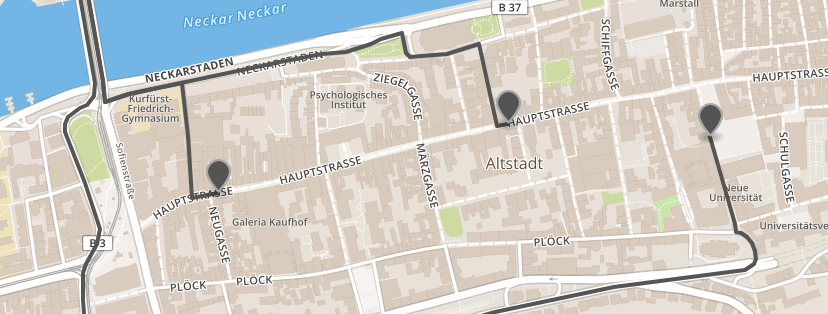
\includegraphics[width = 0.95\textwidth]{../media/Altstadt_emergency.png} \\
\caption{Emergency Routing}
\label{fig:alteme}
\end{subfigure}
\begin{subfigure}{0.49\textwidth}
\centering
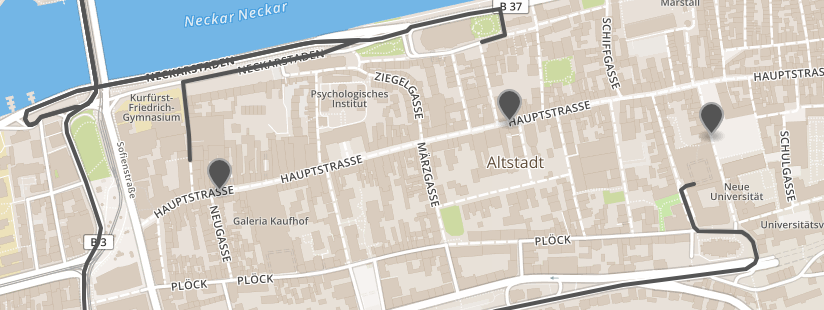
\includegraphics[width = 0.95\textwidth]{../media/Altstadt_car.png} \\
\caption{ORS-Car Routing}
\label{fig:altcar}
\end{subfigure}
\end{figure}

Im Folgenden wurden Isochronen mit der Freiwilligen Feuerwehr Gablingen als Zentrum berechnet (48.454063,10.824415 [Latitude, Longitude]).
Folgende Einstellungen wurden dabei vorgenommen:

- Distanz: 5 min
- Intervall: 1 min
- Maximale Geschwindigkeit: 80 km/h für Löschfahrzeug und HGV; 130 km/h für PKW und Einsatzfahrzeug
- HGV Einstellungen für Löschfahrzeug und HGV: Länge=7m ; Breite= 2.5m; Höhe= 3m; Gewicht= 7.5t

Die Ersten Ergebnisse lieferten zu erwartende Resultate \ref{fig:isochrones}.
Die Emergency Profile konnten in der gleichen Zeit einen größeren Bereich abdecken.

\begin{figure}[h]
\centering
\begin{subfigure}{0.49\textwidth}
\centering
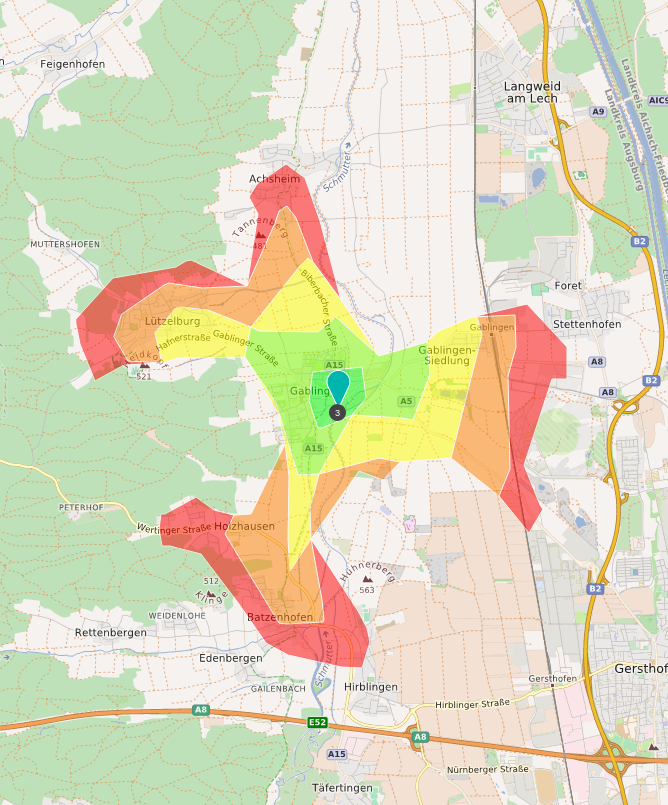
\includegraphics[width = 0.75\textwidth]{../media/isohgv.png} \\
\caption{HGV-Profil}
\label{fig:isohgv}
\end{subfigure}
\begin{subfigure}{0.49\textwidth}
\centering
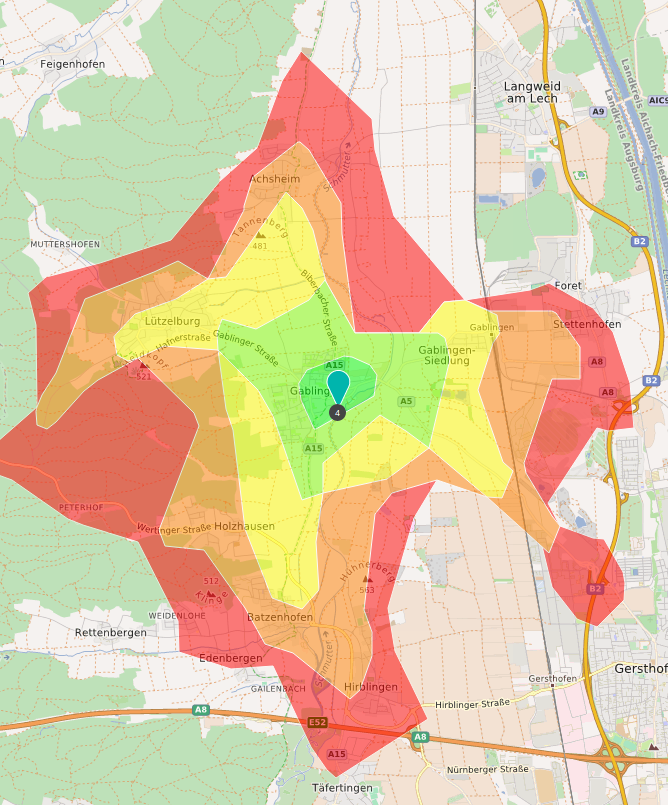
\includegraphics[width = 0.75\textwidth]{../media/isocar.png} \\
\caption{Car-Profil}
\label{fig:isocar}
\end{subfigure}
\begin{subfigure}{0.49\textwidth}
\centering
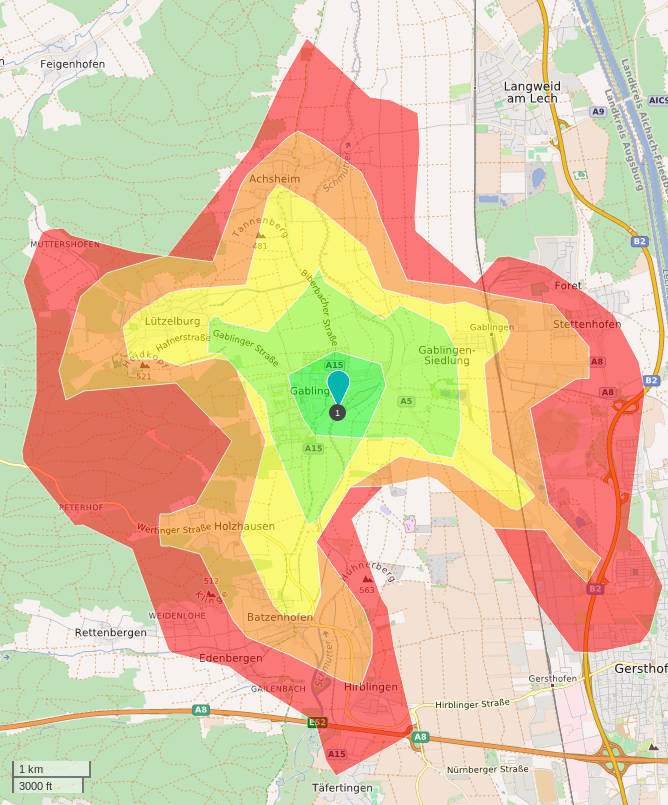
\includegraphics[width = 0.75\textwidth]{../media/isofire.png} \\
\caption{Emergency-Profil -- Löschfahrzeug}
\label{fig:isofire}
\end{subfigure}
\begin{subfigure}{0.49\textwidth}
\centering
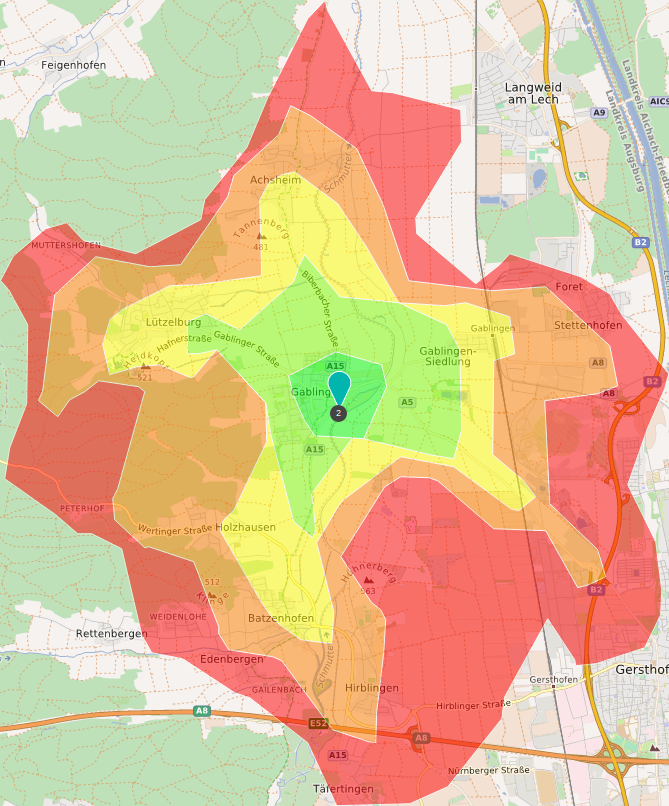
\includegraphics[width = 0.75\textwidth]{../media/isoeme.png} \\
\caption{Emergency-Profil -- Einsatzfahrzeug}
\label{fig:isoeme}
\end{subfigure}
\begin{subfigure}{0.90\textwidth}
\centering
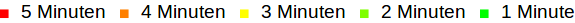
\includegraphics[width = 0.75\textwidth]{../media/legendiso.png} \\
\end{subfigure}
\caption{Ergebnis Isochronen}
\label{fig:isochrones}
\end{figure}

\todo{
mehr Text zu Isochronen? 
erreichbarkeits gebiet tabelle ?
eingehen auf eingeschlossene gebiete?
}

Nach einer Testfahrt der FFL wurde allerdings schnell klar, dass die Ergebnisse nicht im realistischen Bereich liegen.
In fünf Minuten konnte das Löschfahrzeug auf der Einsatzfahrt vom Startpunkt in Gablingen Richtung Muttershofen nur den nordwestlichen Rand von Lützelburg erreichen.
Das Profil kam für das Löschfahrzeug sogar über Muttershofen hinaus.



Um genaue Anpassungen am Backend vorzunehmen wurde eine weitere Testfahrt durchgeführt, bei der für jede volle Minute der Aufenthaltsort des Fahrzeuges markiert wurde (Abb. \ref{fig:drive1}).
Diese Angaben wurden mit den bisherigen Rückgabewerten des Profils verglichen.
Wie aus der Gesamtdauer für die Strecke in Tabelle \ref{tab:driveinit} ersichtlich, ist das Emergency Profil ungefähr 90 Sekunden zu schnell.

\begin{figure}[h]
\centering
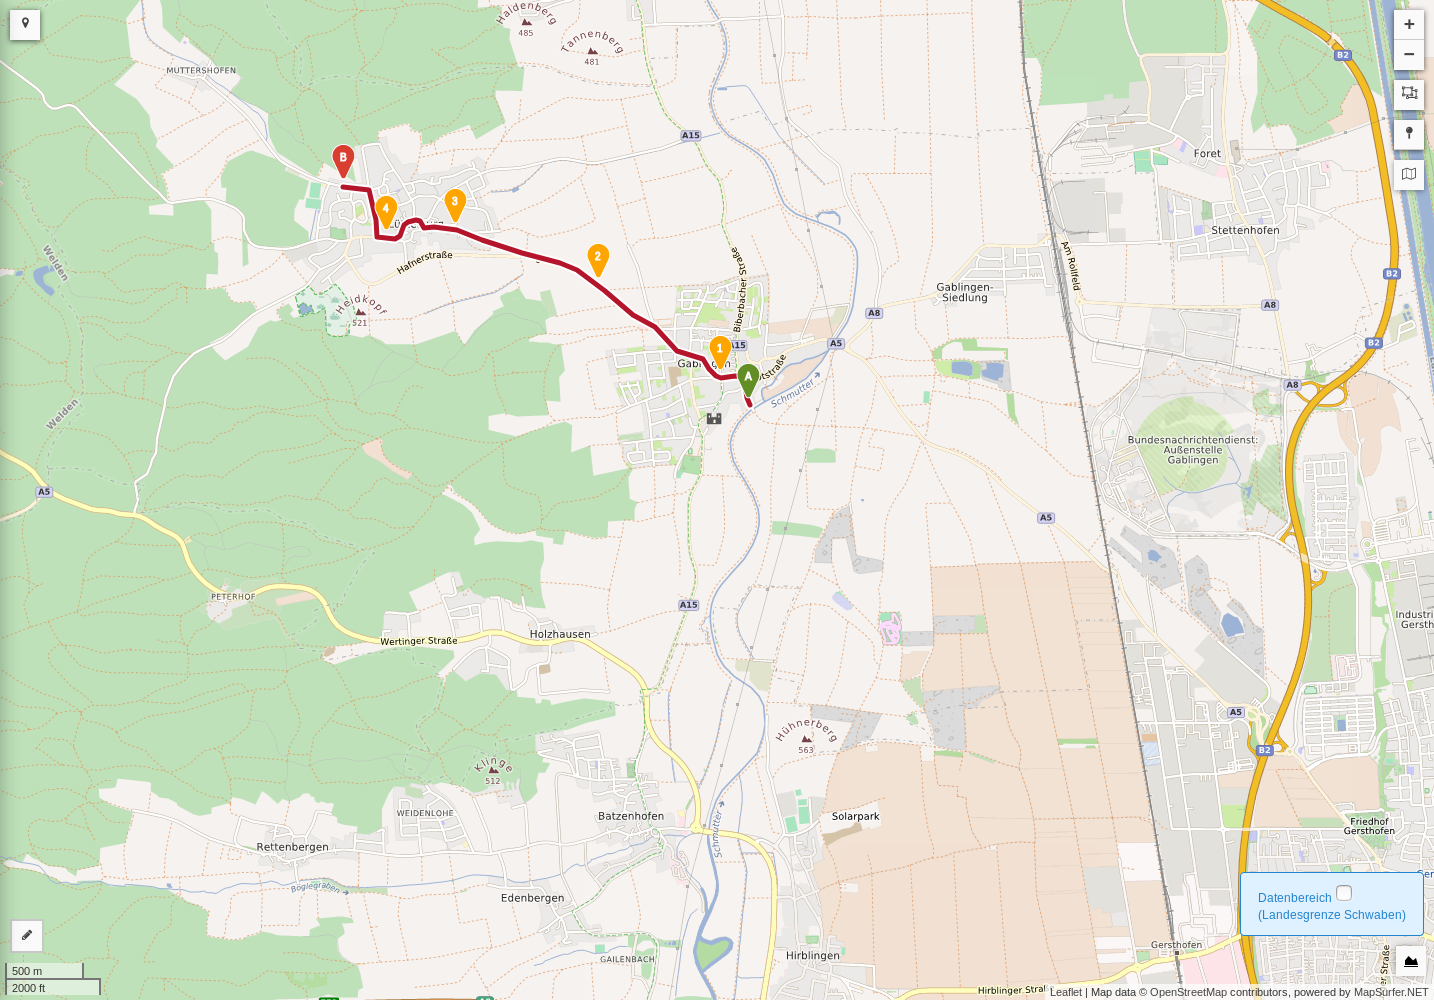
\includegraphics[width = 0.7 \textwidth]{../media/Fahrt1.png} \\
\caption{Testfahrt 1}
\label{fig:drive1}
\end{figure}

\begin{table}[]
\centering
\caption{Fahrt 1 -- 1. Auswertung}
\label{tab:driveinit}
\begin{tabular}{|l|r|r|r|r|r|}
\hline
Wegpunkt                               & \multicolumn{1}{c|}{1} & \multicolumn{1}{c|}{2} & \multicolumn{1}{c|}{3} & \multicolumn{1}{c|}{4} & \multicolumn{1}{c|}{B}  \\ \hline
Distanz                                & 363,2 m                & 1352,8 m               & 2331,9 m               & 2862,3 m               & 3387,3 m               \\ \hline
Fahrtzeit (Profil)                     & 28,6 s                 & 88,7 s                 & 139,4 s                & 177,6 s                & 209,8 s                \\ \hline
Fahrtzeit (Testfahrt)                  & 60,0 s                 & 120,0 s                & 180,0 s                & 240,0 s                & 300,0 s                \\ \hline
Fahrtzeit Abschnitt                    & 28,6 s                 & 60,1 s                 & 50,7 s                 & 38,2 s                 & 32,2 s                 \\ \hline
Fahrtzeit Abschnitt (Testfahrt)        & 60,0 s                 & 60,0 s                 & 60,0 s                 & 60,0 s                 & 60,0 s                 \\ \hline
Geschwindigkeit                        & 45,7 km/h              & 59,3 km/h              & 69,5 km/h              & 50,0 km/h              & 58,7 km/h              \\ \hline
Geschwindigkeit (Testfahrt)            & 21,8 km/h              & 59,4 km/h              & 58,7 km/h              & 31,8 km/h              & 31,5 km/h              \\ \hline
\end{tabular}
\end{table}

Die Vermutung liegt nahe, dass die große Differenz aufgrund der fehlenden Beschleunigungs- und Bremszeiten auftritt.
Bisher wird von graphhopper bei der Berechnung der Fahrzeit lediglich 90$\%$ des für ein Segment vorgegebenen Geschwindigkeitslimits verwendet.
Damit soll sichergestellt sein, dass die Geschwindigkeitsbegrenzung auf jedenfall eingehalten wird.
Dieser Faktor wurde für das Emergency Profil entfernt.
Es wird also ein Straßensegment auf dem 50 km/h gefahren werden darf über die komplette Distanz bisher auch mit 50 km/h gefahren.
In der Realität braucht ein Fahrzeug dieser Größenordnung aber einige Sekunden um diese Geschwindigkeit aus dem Stand zu erreichen.
Die selbe Situation besteht für Bremsvorgänge.
Es bestehen also drei Szenarien auf einer Fahrt, welche nach festgelegter Route einen Einfluss auf die Fahrzeit haben.
Das sind der Start, ein Abbiegevorgang (engl.: Turn) und die Ankunft.
Es gibt selbstverständlich noch mehr Faktoren die zum Beispiel andere Verkehrsteilnehmer betreffen, aber die drei genannten Szenarien sind bereits aus der Routenführung ersichtlich und werden definitiv bei jeder Fahrt auftreten\footnote{Wenn die Fahrt nur geradeaus geht ist auch kein Abbiegevorgang dabei}.

Anhand dieser Idee wurde eine weitere Java-Klasse \texttt{AccelerationWeighting} in der die zusätzliche Zeit für diese Szenarien berechnet wird implementiert (\ref{sec:anhang}).
Diese Klasse soll zwei Funktionen erfüllen.
Zum einen muss bereits bei der Suche nach dem schnellsten Weg im Gegensatz zu geraden Strecken zusätzliche Zeit für Turns mit einfließen.
Zum Anderen müssen bei der Berechnung der Fahrzeit Start-, Ankunfts- und Turnzeit mit berücksichtigt werden.

Es stellt sich die Frage, wie eine Turn auf dem Graphen identifiziert werden kann.
Die Änderung des Straßennamens ist sicherlich eine Möglichkeit viele Abbiegevorgänge abzudecken.
Allerdings ist nicht immer ein Straßenname vorhanden und nicht immer bedeutet der Wechsel des Straßennamens, dass in diese Straße eingebogen werden muss.
Eine bessere Lösung bietet die Ausrichtung der Straßensegmente, da hier die Daten auf jeden Fall vorhanden sind.
Deshalb wird in der AccelerationWeighting Klasse an Tower Nodes (also Kreuzungen) der Winkel zwischen dem letzten und dem nächsten Straßensegment berechnet.
Eine Abbiegung bzw.
scharfe Kurve wird durch einen Winkel zwischen 50 und 140 Grad definiert.
Bei einer Routing Abfrage wird in einem solchen Fall das Gewicht der auf die Kurve folgenden Kante erhöht.
Ebenso wird sobald der schnellste Weg ermittelt ist an diesen Stellen die Bremszeit vor der Abbiegung und die Beschleunigungszeit nach der Abbiegung zur Gesamtzeit des folgenden Wegsegmentes addiert.
Der gleiche Vorgang wird für Start und Ziel durchgeführt.
Die addierte Zeit wird als \textit{Penalty} (dt.: Strafe) bezeichnet.

Anhand der vorliegenden Testfahrt wurde das Profil derart kalibriert, dass durch die Penalties für Abbiegungen, Start und Ziel genau die fehlenden 90 Sekunden gebraucht wurden.
Für Start sowie Ankunft wurden 15 und für Abbiegungen 20 Sekunden veranschlagt.

Mit dem neu eingestellten Profil wurde nun erneut ein Request für die erste Testfahrt gesendet.
Wie erwarte brauchte das Profil nun für diesen Weg ebenfalls fast genau fünf Minuten.
In Tabelle \ref{tab:drive11} ist die Differenz zu den einzelnen Minutenmarkern der 1. Testfahrt für diesen Request zu sehen.
Diese Ergebnisse zeigen dass das Profil den ersten Teil der Route zu langsam und den zweiten Teil zu schnell absolviert.

\begin{table}[h]
\centering
\caption{Fahrt 1 -- Fahrzeit}
\label{tab:drive11}
\begin{tabular}{|l|r|r|}
\hline
Wegpunkt & Fahrtzeit & Abweichung \\ \hline 
1min & 78,3 s & $+18,3$ \\
2min & 138.5 s & $+18,5$ \\
3min & 188.5 s & $+8,5$ \\
4min & 226.7 s & $-3,3$ \\
5min & 298.9 s & $-1,1$ \\
\hline
\end{tabular}
\end{table}

Diese Kalibrierung wurde an zwei weiteren Testfahrten (Abb. \ref{fig:drive2} und \ref{fig:drive3}) vom selben Ausgangspunkt überprüft.

In den Tabellen \ref{tab:drive2} und \ref{tab:drive3} ist zu sehen, das 8 von 10 Wegpunkten um mehr als 20 Sekunden, in 3 Fällen sogar 40 Sekunden zu spät erreicht werden.
Mit den Ergebnissen dieser Testfahrten steht fest: das Profil ist noch erheblich zu langsam und die Penalties zu hoch.

\begin{figure}[h]
\centering
\caption{Testfahrt 2}
\label{fig:drive2}
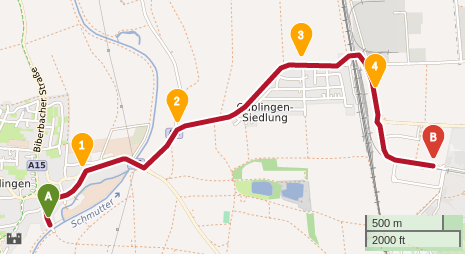
\includegraphics[width = 0.70 \textwidth]{../media/Fahrt2crop.png} \\
\end{figure}

\begin{table}[]
\centering
\caption{Fahrt 2 -- Fahrzeit}
\label{tab:drive2}
\begin{tabular}{|l|r|r|}
\hline
Wegpunkt & Fahrtzeit & Abweichung \\ \hline 
1min & 86.6 $s$ & $+26.6 s$ \\
2min & 149.9 $s$ & $+29.9 s$ \\
3min & 207.5 $s$ & $+27.5 s$ \\
4min & 253.5 $s$ & $+13.5 s$ \\
5min & 318.6 $s$ & $+18.6 s$ \\
\hline
\end{tabular}
\end{table}


\begin{figure}[h]
\centering
\caption{Testfahrt 3}
\label{fig:drive3}
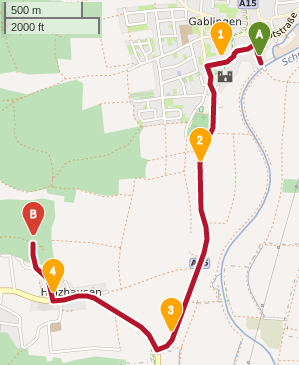
\includegraphics[width = 0.40 \textwidth]{../media/Fahrt3crop.png} \\
\end{figure}

\begin{table}[]
\centering
\caption{Fahrt 3 -- Fahrzeit}
\label{tab:drive3}
\begin{tabular}{|l|r|r|}
\hline
Wegpunkt & Fahrtzeit & Abweichung \\ \hline 
1min: &  89.8 s & $+29.8s$ \\
2min: &  162.4 s & $+42.4$ \\
3min: &  213 s & $+33$ \\
4min: &  282.3 s & $+42.3$ \\
5min: &  343.9 s & $+43.9$ \\
\hline
\end{tabular}
\end{table}

Die Penalties für Start und Ankunft wurden für die folgenden Analysen um die Hälfte reduziert und lagen somit bei 7,5 Sekunden.
Turnpenalties wurden auf 16 Sekunden reduziert.

Mit der neuen Gewichtung wurden die Requests für die drei Testfahrten erneut gesendet und mit den Minuten-Markierungen der wirklich benötigten Zeiten verglichen.
Die Ergebnisse sind der Tabelle \ref{tab:all} zu entnehmen.

\begin{table}[]
\centering
\caption{Fahrt 1,2,3 -- 2. Auswertung}
\label{tab:all}
\begin{tabular}{|l|r|r|r|r|r|r|}
\hhline{~|-|-|-|-|-|-}
\multicolumn{1}{l|}{} & \multicolumn{2}{c|}{Fahrt 1} & \multicolumn{2}{c|}{Fahrt 2} & \multicolumn{2}{c|}{Fahrt 3} \\ \hline
Wegpunkt & Fahrtzeit & Abweichung & Fahrtzeit & Abweichung & Fahrtzeit & Abweichung \\ \hline 
1min & 59.5 & -0.5 & 67.6 & +7.6 & 70.8 & +10.8  \\
2min & 119.5 & -0.5 & 126.9 & +6.9 & 139.4 & +19.4  \\
3min & 169.5 & -10.5 & 184.5 & +4.5 & 190 & +10  \\
4min & 207.7 & -32.2 & 230.5 & -10.5 & 255.2 & +15.2  \\
5min & 271.9 & -28.1 & 291.6 & -8.4 & 312.9 & +12.9   \\
\hline
\end{tabular}
\end{table}


Um die Testfahrten genauer analysieren zu können, wurde das Backend um bisher fehlende Funktionen für die Rückgabe von zusätzlichen Informationen.
Dabei wurden die Speicherobjekte für Wegtypen und Wegoberfläche hinzugefügt und zusätzlich die Höheninformationen der Punte zurückgegeben.
Im Frontend konnten dadurch nun die Wegtypen und Wegoberfächen aber auch die Steigung und somit auch ein Höhenprofil angezeigt werden.
Außerdem wurde ein Feature zur Darstellung der Höchstgeschwindigkeit der einzelnen Streckensegmente eingebaut.